
\documentclass[border=8pt, multi, tikz]{standalone}
\usepackage{import}
\subimport{../../../layers/}{init}
\usetikzlibrary{positioning}
\usetikzlibrary{3d} %for including external image

\def\ConvColor{rgb:yellow,5;red,2.5;white,5}
\def\ConvReluColor{rgb:yellow,5;red,5;white,5}
\def\PoolColor{rgb:red,1;black,0.3}
\def\UnpoolColor{rgb:blue,2;green,1;black,0.3}
\def\ConcatColor{rgb:blue,1;red,1;white,0.3}
\def\FcColor{rgb:blue,5;red,2.5;white,5}
\def\FcReluColor{rgb:blue,5;red,5;white,4}
\def\SoftmaxColor{rgb:pink,5;white,1}

\newcommand{\copymidarrow}{\tikz \draw[-Stealth,line width=0.8mm,draw={rgb:blue,4;red,1;green,1;black,3}] (-0.3,0) -- ++(0.3,0);}

\begin{document}
\begin{tikzpicture}
\tikzstyle{connection}=[ultra thick,every node/.style={sloped,allow upside down},draw=\edgecolor,opacity=0.7]
\tikzstyle{copyconnection}=[ultra thick,every node/.style={sloped,allow upside down},draw={rgb:blue,4;red,1;green,1;black,3},opacity=0.7]

\node[canvas is zy plane at x=0] (net_in) at (-3,0,0)
    {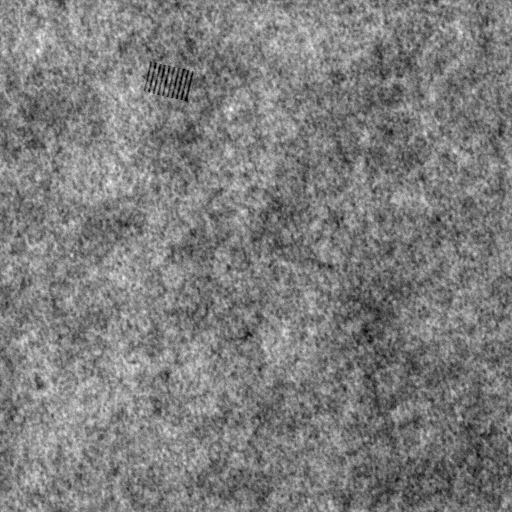
\includegraphics[
        width=6.5cm,
        height=6.5cm
    ]{Class5_0978.PNG}};

\pic[shift={ (-1.5,0,0) }] at (0,0,0)
    {RightBandedBox={
        name=ccr_b1,
        caption= ,
        xlabel={{ 32, 32 }},
        zlabel=512,
        fill=\ConvColor,
        bandfill=\ConvReluColor,
        height=32,
        width={ 2.5 , 2.5 },
        depth=32
        }
    };

\pic[shift={ (1.5,0,0) }] at (ccr_b1-east)
    {Box={
        name=pool_b1,
        caption= ,
        fill=\PoolColor,
        opacity=0.5,
        xlabel={{32, }},
        zlabel=256,
        height=22,
        width=2.5,
        depth=22
        }
    };

\draw [connection]  (ccr_b1-east)    -- node {\midarrow} (pool_b1-west);

\pic[shift={ (2,0,0) }] at (pool_b1-east)
    {RightBandedBox={
        name=ccr_b2,
        caption= ,
        xlabel={{ 32, 32 }},
        zlabel=256,
        fill=\ConvColor,
        bandfill=\ConvReluColor,
        height=22,
        width={ 2.5 , 2.5 },
        depth=22
        }
    };

\pic[shift={ (1.3,0,0) }] at (ccr_b2-east)
    {Box={
        name=pool_b2,
        caption= ,
        fill=\PoolColor,
        opacity=0.5,
        xlabel={{32, }},
        zlabel=128,
        height=15,
        width=2.5,
        depth=15
        }
    };

\draw [connection]  (ccr_b2-east)    -- node {\midarrow} (pool_b2-west);

\draw [connection]  (pool_b1-east)    -- node {\midarrow} (ccr_b2-west);

\pic[shift={ (2,0,0) }] at (pool_b2-east)
    {RightBandedBox={
        name=ccr_b3,
        caption= ,
        xlabel={{ 64, 64 }},
        zlabel=128,
        fill=\ConvColor,
        bandfill=\ConvReluColor,
        height=15,
        width={ 3.5 , 3.5 },
        depth=15
        }
    };

\pic[shift={ (1.2,0,0) }] at (ccr_b3-east)
    {Box={
        name=pool_b3,
        caption= ,
        fill=\PoolColor,
        opacity=0.5,
        xlabel={{64, }},
        zlabel=64,
        height=10,
        width=3.5,
        depth=10
        }
    };

\draw [connection]  (ccr_b3-east)    -- node {\midarrow} (pool_b3-west);

\draw [connection]  (pool_b2-east)    -- node {\midarrow} (ccr_b3-west);

\pic[shift={ (1.5,0,0) }] at (pool_b3-east)
    {RightBandedBox={
        name=ccr_b4,
        caption= ,
        xlabel={{ 128, 128 }},
        zlabel=64,
        fill=\ConvColor,
        bandfill=\ConvReluColor,
        height=10,
        width={ 4.5 , 4.5 },
        depth=10
        }
    };

\pic[shift={ (0.95,0,0) }] at (ccr_b4-east)
    {Box={
        name=pool_b4,
        caption= ,
        fill=\PoolColor,
        opacity=0.5,
        xlabel={{128, }},
        zlabel=32,
        height=7,
        width=4.5,
        depth=7
        }
    };

\draw [connection]  (ccr_b4-east)    -- node {\midarrow} (pool_b4-west);

\draw [connection]  (pool_b3-east)    -- node {\midarrow} (ccr_b4-west);

\pic[shift={ (1.5,0,0) }] at (pool_b4-east)
    {RightBandedBox={
        name=ccr_b5,
        caption=Bottleneck,
        xlabel={{ 256, 256 }},
        zlabel=32,
        fill=\ConvColor,
        bandfill=\ConvReluColor,
        height=7,
        width={ 7 , 7 },
        depth=8
        }
    };

\draw [connection]  (pool_b4-east)    -- node {\midarrow} (ccr_b5-west);

\pic[shift={ (1.5,0,0) }] at (ccr_b5-east)
    {Box={
        name=unpool_b6,
        caption= ,
        fill=\UnpoolColor,
        opacity=0.5,
        xlabel={{512, }},
        zlabel=64,
        height=10,
        width=1,
        depth=10
        }
    };

\pic[shift={ (0.95,0,0) }] at (unpool_b6-east)
    {Box={
        name=concat_b6,
        caption= ,
        fill=\ConcatColor,
        opacity=0.5,
        xlabel={{512, }},
        zlabel=64,
        height=10,
        width=5.0,
        depth=10
        }
    };

\pic[shift={ (0.95,0,0) }] at (concat_b6-east)
    {RightBandedBox={
        name=ccr_b6,
        caption= ,
        xlabel={{ 512, 512 }},
        zlabel=64,
        fill=\ConvColor,
        bandfill=\ConvReluColor,
        height=10,
        width={ 5.0 , 5.0 },
        depth=10
        }
    };

\draw [connection]  (ccr_b5-east)    -- node {\midarrow} (unpool_b6-west);

\draw [connection]  (unpool_b6-east)    -- node {\midarrow} (concat_b6-west);

\draw [connection]  (unpool_b6-east)    -- node {\midarrow} (ccr_b6-west);

\path (ccr_b4-southeast) -- (ccr_b4-northeast) coordinate[pos=1.25] (ccr_b4-top) ;
\path (concat_b6-south)  -- (concat_b6-north)  coordinate[pos=1.25] (concat_b6-top) ;
\draw [copyconnection]  (ccr_b4-northeast)
-- node {\copymidarrow}(ccr_b4-top)
-- node {\copymidarrow}(concat_b6-top)
-- node {\copymidarrow} (concat_b6-north);

\pic[shift={ (2,0,0) }] at (ccr_b6-east)
    {Box={
        name=unpool_b7,
        caption= ,
        fill=\UnpoolColor,
        opacity=0.5,
        xlabel={{256, }},
        zlabel=128,
        height=15,
        width=1,
        depth=15
        }
    };

\pic[shift={ (1.3,0,0) }] at (unpool_b7-east)
    {Box={
        name=concat_b7,
        caption= ,
        fill=\ConcatColor,
        opacity=0.5,
        xlabel={{256, }},
        zlabel=128,
        height=15,
        width=4.5,
        depth=15
        }
    };

\pic[shift={ (1.3,0,0) }] at (concat_b7-east)
    {RightBandedBox={
        name=ccr_b7,
        caption= ,
        xlabel={{ 256, 256 }},
        zlabel=128,
        fill=\ConvColor,
        bandfill=\ConvReluColor,
        height=15,
        width={ 4.5 , 4.5 },
        depth=15
        }
    };

\draw [connection]  (ccr_b6-east)    -- node {\midarrow} (unpool_b7-west);

\draw [connection]  (unpool_b7-east)    -- node {\midarrow} (concat_b7-west);

\draw [connection]  (unpool_b7-east)    -- node {\midarrow} (ccr_b7-west);

\path (ccr_b3-southeast) -- (ccr_b3-northeast) coordinate[pos=1.25] (ccr_b3-top) ;
\path (concat_b7-south)  -- (concat_b7-north)  coordinate[pos=1.25] (concat_b7-top) ;
\draw [copyconnection]  (ccr_b3-northeast)
-- node {\copymidarrow}(ccr_b3-top)
-- node {\copymidarrow}(concat_b7-top)
-- node {\copymidarrow} (concat_b7-north);

\pic[shift={ (2.5,0,0) }] at (ccr_b7-east)
    {Box={
        name=unpool_b8,
        caption= ,
        fill=\UnpoolColor,
        opacity=0.5,
        xlabel={{128, }},
        zlabel=256,
        height=22,
        width=1,
        depth=22
        }
    };

\pic[shift={ (1.5,0,0) }] at (unpool_b8-east)
    {Box={
        name=concat_b8,
        caption= ,
        fill=\ConcatColor,
        opacity=0.5,
        xlabel={{128, }},
        zlabel=256,
        height=22,
        width=3.5,
        depth=22
        }
    };

\pic[shift={ (1.5,0,0) }] at (concat_b8-east)
    {RightBandedBox={
        name=ccr_b8,
        caption= ,
        xlabel={{ 128, 128 }},
        zlabel=256,
        fill=\ConvColor,
        bandfill=\ConvReluColor,
        height=22,
        width={ 3.5 , 3.5 },
        depth=22
        }
    };

\draw [connection]  (ccr_b7-east)    -- node {\midarrow} (unpool_b8-west);

\draw [connection]  (unpool_b8-east)    -- node {\midarrow} (concat_b8-west);

\draw [connection]  (unpool_b8-east)    -- node {\midarrow} (ccr_b8-west);

\path (ccr_b2-southeast) -- (ccr_b2-northeast) coordinate[pos=1.25] (ccr_b2-top) ;
\path (concat_b8-south)  -- (concat_b8-north)  coordinate[pos=1.25] (concat_b8-top) ;
\draw [copyconnection]  (ccr_b2-northeast)
-- node {\copymidarrow}(ccr_b2-top)
-- node {\copymidarrow}(concat_b8-top)
-- node {\copymidarrow} (concat_b8-north);

\pic[shift={ (3,0,0) }] at (ccr_b8-east)
    {Box={
        name=unpool_b9,
        caption= ,
        fill=\UnpoolColor,
        opacity=0.5,
        xlabel={{64, }},
        zlabel=512,
        height=32,
        width=1,
        depth=32
        }
    };

\pic[shift={ (1.7,0,0) }] at (unpool_b9-east)
    {Box={
        name=concat_b9,
        caption= ,
        fill=\ConcatColor,
        opacity=0.5,
        xlabel={{64, }},
        zlabel=512,
        height=32,
        width=2.5,
        depth=32
        }
    };

\pic[shift={ (1.7,0,0) }] at (concat_b9-east)
    {RightBandedBox={
        name=ccr_b9,
        caption= ,
        xlabel={{ 64, 64 }},
        zlabel=512,
        fill=\ConvColor,
        bandfill=\ConvReluColor,
        height=32,
        width={ 2.5 , 2.5 },
        depth=32
        }
    };

\draw [connection]  (ccr_b8-east)    -- node {\midarrow} (unpool_b9-west);

\draw [connection]  (unpool_b9-east)    -- node {\midarrow} (concat_b9-west);

\draw [connection]  (unpool_b9-east)    -- node {\midarrow} (ccr_b9-west);

\path (ccr_b1-southeast) -- (ccr_b1-northeast) coordinate[pos=1.25] (ccr_b1-top) ;
\path (concat_b9-south)  -- (concat_b9-north)  coordinate[pos=1.25] (concat_b9-top) ;
\draw [copyconnection]  (ccr_b1-northeast)
-- node {\copymidarrow}(ccr_b1-top)
-- node {\copymidarrow}(concat_b9-top)
-- node {\copymidarrow} (concat_b9-north);

\pic[shift={(2,0,0)}] at (ccr_b9-east)
    {Box={
        name=soft1,
        caption=Sigmoid,
        xlabel={{ 1, }},
        zlabel=512,
        fill=\SoftmaxColor,
        height=32,
        width=1,
        depth=32
        }
    };

\draw [connection]  (ccr_b9-east)    -- node {\midarrow} (soft1-west);

\end{tikzpicture}
\end{document}
